\documentclass[11pt,a4paper]{article}
\usepackage[margin=2.1cm]{geometry}
\usepackage{booktabs}
\usepackage{tabularx}
\usepackage{longtable}
\usepackage{array}
\usepackage{graphicx}
\usepackage{pdflscape}
\usepackage{tikz}
\usepackage{tikz-timing}
\usetikzlibrary{positioning,arrows.meta}
\usepackage{xcolor}
\usepackage{enumitem}
\usepackage{listings}
\usepackage{caption}
\usepackage[hidelinks]{hyperref}
\usepackage{fancyhdr}

\definecolor{codebg}{HTML}{F4F7F6}
\definecolor{teal}{HTML}{0B7670}
\newcommand{\sig}[1]{\texttt{#1}}
\setlist{itemsep=2pt,topsep=4pt}
\setlength{\parskip}{4pt}
\setlength{\parindent}{0pt}
\lstset{basicstyle=\ttfamily\small,backgroundcolor=\color{codebg},frame=none,xleftmargin=6pt,xrightmargin=6pt,aboveskip=6pt,belowskip=6pt,columns=fullflexible,keepspaces=true,showstringspaces=false}
\tikzset{timing/d/text/.style={font=\scriptsize},timing/rowdist=2.6ex}

\pagestyle{fancy}
\fancyhf{}
\lhead{\small Paul Vincent Bezzina | ProEm - Open Source Protocol Emulator}
\rhead{\small Design reference v1.0}
\cfoot{\small\thepage}

\title{ProEm: Protocol Emulator ASIC\\\large Design Reference}
\author{Paul Vincent Bezzina}
\date{26 September 2026}

\begin{document}
\maketitle
\thispagestyle{fancy}

\begin{center}
\begin{tabular}{@{}ll@{}}
\toprule
Process & IHP SG13G2 130\,nm, through Tiny Tapeout (6 $\times$ 2 tiles) \\
System clock & 50\,MHz (60\,MHz for 10BASE-T transmit) \\
Channels & 2 independent protocol channels, A and B \\
Host link & UART in (auto-baud), UART out (rate set by \sig{LINK}) \\
Standards verified & UART, SPI (controller and target), I\textsuperscript{2}C (controller), PS/2, \\
 & 10BASE-T receive, Manchester transmit, USB low speed receive and transmit \\
Logic & 13,144 cells after synthesis, 17,135 after place and route (72\,\% utilisation) \\
Timing & closed after routing: 14.1\,ns worst path at 1.08\,V, 125\,$^\circ$C (20\,ns budget) \\
Instruction set & ISA v0.4 (separate document: \emph{ProEm Instruction Set}) \\
\bottomrule
\end{tabular}
\end{center}

\tableofcontents
\newpage

\section{Overview}

ProEm is an open-source protocol emulator ASIC. The chip lets an RP2040 speak many serial protocols through one piece of hardware. The RP2040 does not bit-bang anything. It describes a frame to the chip in a few instruction bytes: how the frame starts, which fields follow, which way each field goes, how the frame ends, how the line is coded and where the bit clock comes from. The chip then runs the frame at up to one bit per system clock, with exact timing, and sends back what it received together with a status for every frame.

The design has four parts:
\begin{enumerate}
\item \textbf{Host side.} A UART receiver with auto-baud feeds the control unit, which decodes ISA v0.4 instructions into registered configuration writes. A return path sends received data, frame status and link events back on a second UART.
\item \textbf{Input pipeline.} Every input pin passes through two synchroniser flip-flops and one more register before any logic uses it.
\item \textbf{Two channels.} Each channel has a host FIFO for write data, a \emph{frame chain} that runs the frame, an \emph{entry dispatcher}, and a \emph{line codec} that turns pins into bits and ticks, and bits into pin levels.
\item \textbf{Outputs.} Each channel drives a data output, a pair output (the complement, for USB D$-$), a clock output and a select output, each with an output enable. Bidirectional pads are read back through the input pins.
\end{enumerate}

The two channels run at the same time. That is how the chip does SPI full duplex (one channel writes MOSI, the other reads MISO), UART receive and transmit together, or a transmitter looped into a receiver for self-test.

\begin{landscape}
\begin{figure}[p]
\centering
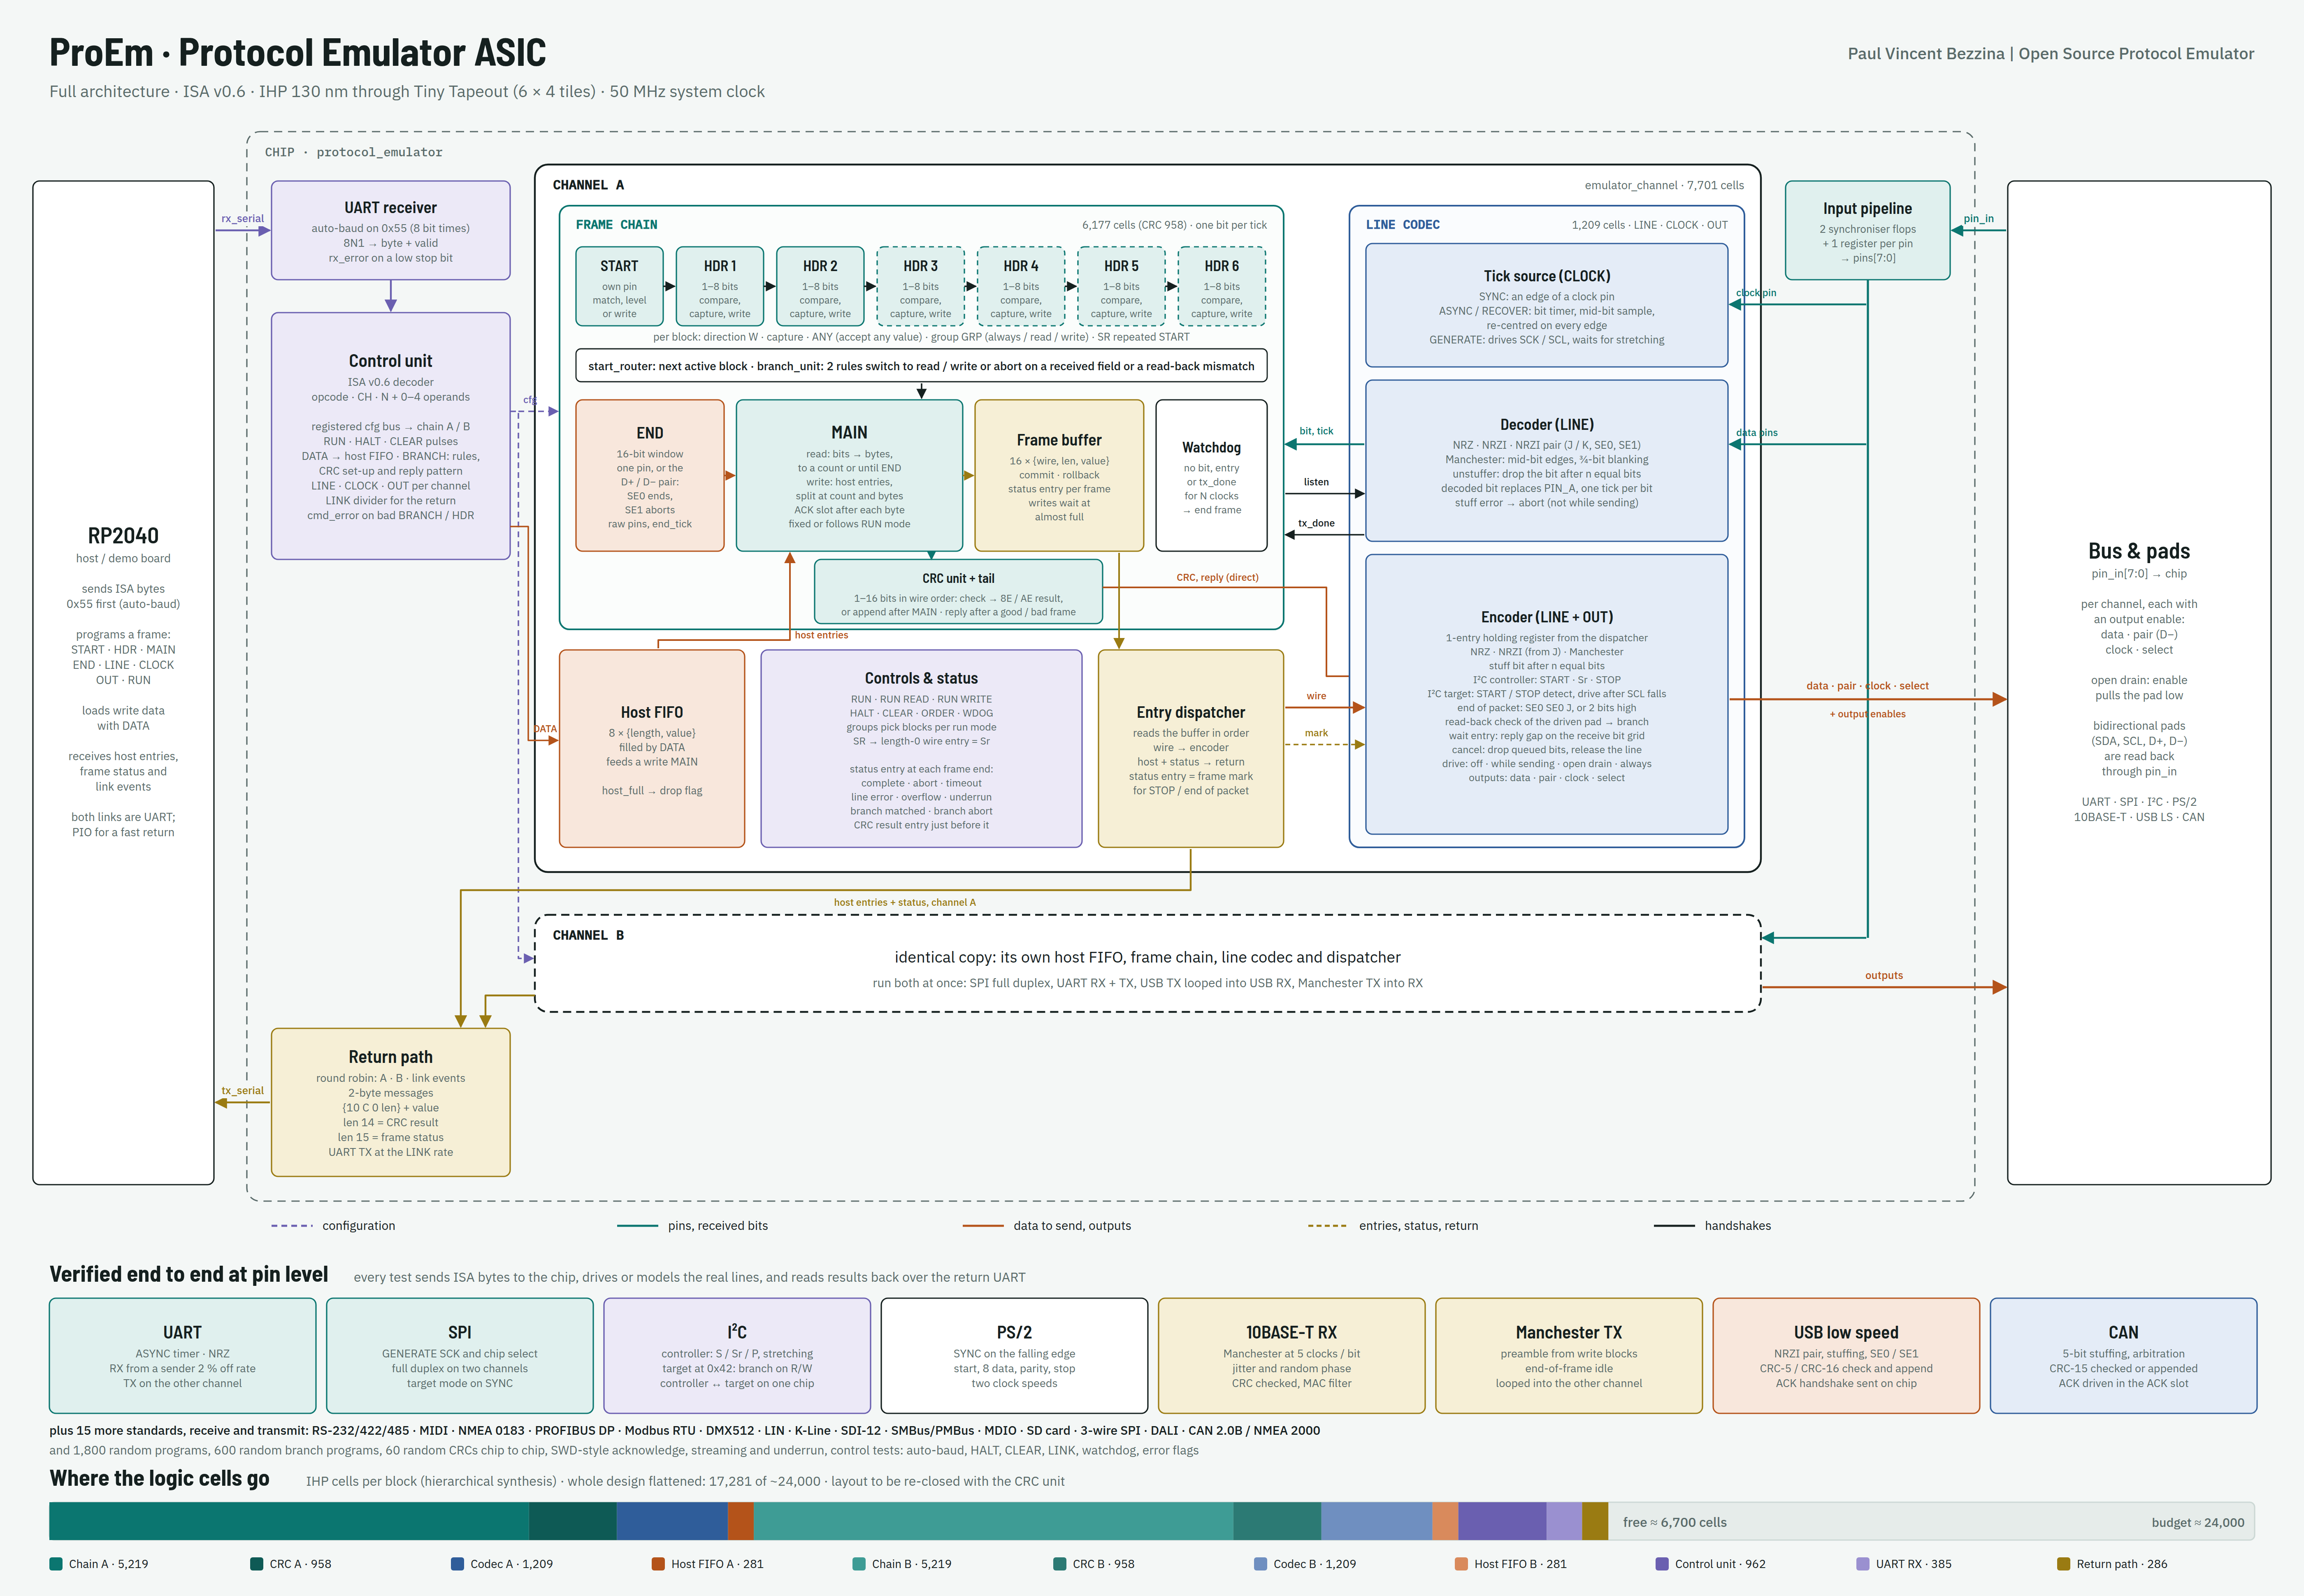
\includegraphics[width=\linewidth]{protocol_emulator_architecture.png}
\caption{The whole chip. Channel A is shown in full; channel B is an identical copy.}
\label{fig:arch}
\end{figure}
\end{landscape}

\section{Top-level interface}

The top module is \sig{protocol\_emulator}. Its ports are generic; the Tiny Tapeout wrapper maps them onto \sig{ui\_in}, \sig{uo\_out} and the bidirectional \sig{uio} pins.

\begin{center}
\begin{tabularx}{\linewidth}{@{}l l >{\raggedright\arraybackslash}X@{}}
\toprule
Port & Dir & Meaning \\
\midrule
\sig{clk}, \sig{rst\_n} & in & System clock and active-low asynchronous reset \\
\sig{rx\_serial} & in & Instruction bytes from the RP2040, 8N1. The first byte after reset must be \texttt{0x55} \\
\sig{pin\_in[7:0]} & in & Protocol input pins, shared by both channels \\
\sig{tx\_serial} & out & Return UART to the RP2040 \\
\sig{data\_out\_x}, \sig{data\_oe\_x} & out & Channel x data output and output enable. In open-drain mode \sig{out} is 0 and \sig{oe} pulls the pad low \\
\sig{pair\_out\_x}, \sig{pair\_oe\_x} & out & Complement of the data output (USB D$-$) \\
\sig{clock\_out\_x}, \sig{clock\_oe\_x} & out & Generated clock (SCK, SCL) \\
\sig{select\_out\_x} & out & Chip select: active from the frame's START until its last bit has gone out \\
\sig{armed\_x}, \sig{host\_full\_x}, \sig{baud\_locked} & out & Debug status \\
\bottomrule
\end{tabularx}
\end{center}

\paragraph{Pads.} A bidirectional line such as SDA is a pad driven by \sig{data\_out}/\sig{data\_oe} and read back on one of the \sig{pin\_in} bits. I\textsuperscript{2}C uses open drain on both SDA and SCL, so the pads need external pull-ups. USB low speed needs 1.5\,k$\Omega$ from D$-$ to 3.3\,V when the chip is the device, and the pad voltage must reach 2.8\,V or a transceiver is needed.

\paragraph{Input latency.} The pipeline adds three clocks between a pad and the logic. Every pin is delayed equally, so a data pin and a clock pin stay aligned.

\section{Blocks}

\subsection{UART receiver and auto-baud (\sig{uart\_rx})}

After reset the receiver waits for the first falling edge, then counts clocks until the fifth falling edge. For \texttt{0x55} those five edges are exactly 8 bit times apart, so the clocks per bit are the count divided by 8. The receiver then waits for the stop bit and becomes a normal 8N1 receiver at that rate. The sync byte is not passed on. A byte whose stop bit is low raises \sig{rx\_error}. The measured rate is also the default rate of the return UART.

\subsection{Control unit (\sig{control\_unit})}

The control unit reads an opcode byte \texttt{\{OP, CH, N\}}, collects 0--4 operand bytes, and in one further clock turns the instruction into:
\begin{itemize}
\item a write on the shared configuration bus with a write enable for channel A or B (\sig{START}, \sig{HDR}, \sig{MAIN}, \sig{END}, \sig{WDOG}, \sig{ORDER});
\item a pulse: \sig{RUN} with its mode, \sig{HALT} or \sig{CLEAR};
\item a host FIFO write (\sig{DATA});
\item a register update: \sig{LINE}, \sig{CLOCK} and \sig{OUT} per channel, \sig{LINK} for the return link.
\end{itemize}
Every output is a register, so the configuration bus forms a pipeline stage and the decode logic is never in a channel's timing path. \sig{START} patterns are given as plain numbers; the control unit aligns them for the channel's bit order. Reserved opcodes and \sig{HDR 0}/\sig{HDR 7} raise \sig{cmd\_error}.

\subsection{Frame chain (\sig{frame\_chain})}

The frame chain is the frame engine: one START block, up to six header blocks and one MAIN block, run strictly in order, one bit per tick.

\begin{itemize}
\item \textbf{START} slides an 8-bit window over its own pin and matches a pattern of 1--8 bits; with 0 bits it waits for a level (SPI chip select); as a write block it sends its value when \sig{RUN} starts the frame.
\item \textbf{Headers} each compare, capture or send a 1--8 bit field. Each has a group (always, read runs, write runs) and an optional repeated START before it.
\item \textbf{start\_router} enables the next active block after the previous one succeeds. It skips unconfigured blocks and blocks whose group is not in the current run mode.
\item \textbf{MAIN} reads bits into bytes, to a count or until END; or writes host entries, splitting them at the frame's bit count and, with the ACK slot on, at byte edges. After each byte it can add one bit the other way (I\textsuperscript{2}C ACK). Its direction is fixed or follows the run mode.
\item \textbf{END} slides a 16-bit window over one raw pin, or over the D+/D$-$ pair compare: both low (SE0) is a 1, both high (SE1) aborts with a line error. After an abort, START waits until END has matched again, so it never searches inside the rest of a rejected frame.
\item \textbf{Watchdog} ends a frame when no bit, host entry or sent entry is seen for a set number of clocks.
\item \textbf{Frame buffer} holds 16 entries \texttt{\{wire, length, value\}}. Written values are released at once; captured values are released when MAIN starts and dropped on abort. At the end of every frame the chain adds a \emph{status entry} (length 15) with complete, abort, timeout, line error and overflow flags.
\end{itemize}

Read blocks only take ticks once every bit written ahead of them has left the chip (\sig{line\_free}), so a frame can send a request and then read the reply. Write blocks wait when the buffer is almost full, so written bits are never lost; received entries that arrive with the buffer full are dropped and the frame's status has the overflow flag.

\subsection{Host FIFO and entry dispatcher}

The host FIFO holds 8 \texttt{\{length, value\}} entries loaded by \sig{DATA} and feeds a write MAIN. A \sig{DATA} arriving while it is full is dropped and reported as a link event.

The entry dispatcher reads the frame buffer in order. Wire entries go to the codec's encoder; host entries and status entries go to the return path. When a status entry reaches the head, every bit of that frame has already been handed to the encoder, so the dispatcher gives the encoder a \emph{frame mark} at that moment. The encoder uses it to send the I\textsuperscript{2}C STOP or the end of packet at exactly the right place.

\subsection{Line codec (\sig{line\_codec})}

The codec sits between the pins and the frame chain. \sig{CLOCK} chooses the tick source, \sig{LINE} the line code, \sig{OUT} the output behaviour.

\paragraph{Tick source.}
\begin{itemize}
\item \textbf{SYNC}: a tick on the rising, falling or both edges of a clock pin (SPI target, PS/2, a read-back clock).
\item \textbf{ASYNC / RECOVER}: a bit timer of \sig{DIV} clocks per bit that samples mid-bit and re-centres on every edge of the data line. The decoded bit replaces \sig{LINE}'s \sig{PIN\_A} in the pins the chain sees, with one tick per bit.
\item \textbf{GENERATE}: the codec drives the clock output, \sig{DIV} clocks per half period, only while a bit is waiting to go out or a read block wants one. The sampling edge gives the tick. With open drain it waits for the clock read-back pin to go high, which gives I\textsuperscript{2}C clock stretching.
\end{itemize}

\paragraph{Decoder.} NRZ takes the mid-bit sample. NRZI compares it with the previous one (same = 1). The NRZI pair code reads J/K from D+ and D$-$ and gives no bits during SE0 or SE1. Manchester decodes on the mid-bit edges: the new level is the bit, and edges within $\frac34$ of a bit after an accepted edge are ignored, which skips the boundary edges between equal bits. An unstuffer drops the bit after $n$ equal bits; a stuffed bit with the wrong value aborts the frame with a line error.

\paragraph{Encoder.} It holds one entry from the dispatcher and sends it bit 0 first (the chain has already reversed MSB-first fields). It encodes NRZ, NRZI starting from J, or Manchester, inserts a stuff bit after $n$ equal bits, and continues seamlessly into the next entry. In I\textsuperscript{2}C mode it sends START before a transaction, repeated START for a length-0 entry, and STOP at the frame mark. With end of packet on, the frame mark produces two bit times of SE0 and one of J on a pair, or two bit times high on a single line. \sig{tx\_done} after each entry lets the chain know the line is free.

\begin{figure}[h]
\centering
\begin{tikztimingtable}[timing/slope=0.12,xscale=1.9,yscale=1.1]
UART \texttt{0x48} & 2H 4L H 2L H L 2H \\
 & 2D{idle} D{S} D{0} D{0} D{0} D{1} D{0} D{0} D{1} D{0} 2D{stop} \\
\extracode
\end{tikztimingtable}

\vspace{8pt}
\begin{tikztimingtable}[timing/slope=0.12,xscale=1.9,yscale=1.1]
USB D+ & L 7H 5L \\
USB D$-$ & H 7L 2H 2L H \\
 & D{J} D{0} 6D{six 1s: no change} D{st} D{1} 2D{SE0} D{J} \\
\end{tikztimingtable}

\vspace{8pt}
\begin{tikztimingtable}[timing/slope=0.12,xscale=1.9,yscale=1.1]
Manchester & L 2H 2L H L 2H L \\
 & 2D{1} 2D{0} 2D{1} 2D{1} 2D{0} \\
\end{tikztimingtable}
\caption{Three line codes from the same codec. UART: NRZ, LSB first, start and stop bits. USB low speed: NRZI on D+/D$-$ (a 0 changes the line), a stuff bit (st) after six 1s, then the end of packet. 10BASE-T: Manchester, low-to-high in the middle of the bit = 1.}
\end{figure}

\paragraph{Outputs.} \sig{DRIVE} is off after reset, push-pull while sending, open drain, or push-pull always (with an idle level, for a UART line). The pair output carries the complement. The select output is active from the frame's START until its last bit has gone out.

\subsection{Return path (\sig{return\_path}, \sig{uart\_tx})}

The return path takes host entries and status entries from both channels and link events, in round robin, and sends each as a two-byte message on the return UART at the \sig{LINK} rate (or the auto-baud rate when \sig{LINK} is 0).

\section{Host protocol}

\subsection{Start-up}

\begin{enumerate}
\item Release reset and hold \sig{rx\_serial} high for at least one byte time.
\item Send \texttt{0x55}. The chip measures the rate from it; \sig{baud\_locked} goes high.
\item Optionally send \sig{LINK} to speed up the return link (\texttt{E0 00 04} = 4 clocks per bit, 12.5\,Mbaud at 50\,MHz).
\item Program each channel: \sig{LINE}, \sig{CLOCK}, \sig{OUT}, \sig{ORDER}, \sig{WDOG}, the blocks, then \sig{RUN}.
\end{enumerate}

\sig{CLEAR} returns a channel to its reset state, including its outputs; \sig{HALT} stops a frame and disarms the channel but keeps its program.

\subsection{Return messages}

\begin{center}
\begin{tabularx}{\linewidth}{@{}l l >{\raggedright\arraybackslash}X@{}}
\toprule
First byte & Second & Meaning \\
\midrule
\texttt{10 C 0 LLLL} & value & Host entry from channel \texttt{C}, length 0--8. Length 0 with value \texttt{02} is a NACK from a writing MAIN \\
\texttt{10 C 0 1111} & flags & End of a frame on channel \texttt{C}: bit 0 complete, 1 abort, 2 timeout, 3 line error, 4 overflow \\
\texttt{11 000000} & flags & Link events: bit 0 \sig{rx\_error}, 1 \sig{cmd\_error}, 2 \sig{DATA} dropped on A, 3 on B \\
\bottomrule
\end{tabularx}
\end{center}

A frame's host entries always come before its status message. A simple receiver on the RP2040:

\begin{lstlisting}[language=C]
void on_return_message(uint8_t head, uint8_t value) {
    if ((head & 0xC0) == 0xC0) { link_events(value); return; }
    int chan = (head >> 5) & 1, len = head & 0x0F;
    if (len == 15) frame_done(chan, value);        /* status flags   */
    else           frame_data(chan, len, value);   /* 0..8 bits      */
}
\end{lstlisting}

\subsection{Choosing \sig{RUN} modes}

\begin{itemize}
\item \textbf{Receiving:} plain \sig{RUN} arms the channel; it stays armed after every frame.
\item \textbf{Packets} (USB, Ethernet, I\textsuperscript{2}C transactions): load the data with \sig{DATA}, then \sig{RUN WRITE} or \sig{RUN READ}. The channel starts exactly one frame per \sig{RUN}.
\item \textbf{Streams} (UART transmit): plain \sig{RUN}. The channel also starts a new frame whenever data is waiting.
\end{itemize}

\section{Protocol recipes}

Each recipe lists the instruction bytes. The bytes were produced by the test bench's own encoder, and the same programs (with smaller dividers, to keep simulation short) pass the tests in Section~\ref{sec:verify}. Dividers are for a 50\,MHz clock.


\paragraph{UART receive, 115\,200 baud, channel A.} RX on pin 0. \sig{LINE} none on pin 0; \sig{CLOCK} ASYNC, 434 clocks per bit; START reads the start bit; MAIN reads 8 data bits and the stop bit.
\begin{lstlisting}
A0 00 00   B0 40 00 01 B2   10 01 00 00   30 00 00 09   70
\end{lstlisting}


\paragraph{UART transmit, channel B.} Push-pull output, idle high; START writes the start bit; MAIN writes 9 bits. Each byte is two \sig{DATA} entries: the byte and a stop bit.
\begin{lstlisting}
A8 00 00   B8 40 00 01 B2   D8 E0   18 81 00 00   38 40 00 09
CF 48   C8 01   78                                  ("H", then RUN)
\end{lstlisting}


\paragraph{SPI controller, mode 0, MSB first, full duplex.} Channel A generates SCK (half period 6 clocks) and chip select, writes MOSI from \sig{DATA}. Channel B reads MISO on pin 3, clocked by SCK read back on pin 1, started by chip select read back on pin 2.
\begin{lstlisting}
A: 61   A0 00 00   B0 81 00 00 06   D0 C0   50 0F A0   10 80 00 00   30 40 00 10
B: 69   A8 03 00   B8 01 00 00 00   18 00 02 00   38 03 00 10   78
transfer:   C7 A5   C7 5A   70
\end{lstlisting}


\paragraph{I\textsuperscript{2}C controller, 100\,kHz, register read and write in one program.} Device 0x48, register 0x05. SDA read back on pin 0, SCL on pin 1; open drain with I\textsuperscript{2}C conditions.
\begin{lstlisting}
61   A0 00 00   B0 89 00 00 FA   D0 A4   50 EA 60
10 88 00 90   21 01 00 00   22 88 00 05   23 01 00 00
24 98 80 91   25 11 00 00   30 90 00 10
write:  C7 A1   C7 B2   72        bus: S 90 A 05 A A1 A B2 A P
read:   71                        bus: S 90 A 05 A Sr 91 A d0 A d1 N P
\end{lstlisting}


\paragraph{PS/2 keyboard to host, channel B.} Clock on pin 4 (falling edge), data on pin 5. Each key gives \texttt{\{8, code\}} and \texttt{\{2, parity + stop\}}.
\begin{lstlisting}
A8 05 00   B8 14 00 00 00   18 01 05 00   38 05 00 0A   78
\end{lstlisting}


\paragraph{10BASE-T receive, broadcast frames.} Manchester line on pin 0; END sees the line high for 8 clocks at the end of the frame; return link at 4 clocks per bit.
\begin{lstlisting}
E0 00 04   A0 60 00   B0 C0 40 00 05   10 08 00 D5
21 48 00 FF   22 48 00 FF   23 48 00 FF   24 48 00 FF   25 48 00 FF   26 48 00 FF
30 20 00 00   40 40 00 00 FF   70
\end{lstlisting}


\paragraph{Manchester transmit (6 clocks per bit, a 60\,MHz clock for 10\,Mb/s).} The preamble comes from START and six write headers; MAIN sends up to 8 \sig{DATA} bytes (SFD first); end of packet holds the line high for two bit times.
\begin{lstlisting}
A0 60 00   B0 C0 00 00 06   D0 48   10 88 00 55
21 88 00 55   22 88 00 55   23 88 00 55   24 88 00 55   25 88 00 55   26 88 00 55
30 40 00 40      then DATA entries and RUN WRITE (72)
\end{lstlisting}


\paragraph{USB low speed receive.} D+ on pin 0, D$-$ on pin 1; NRZI pair with unstuffing; END on the pair, 2 bit times of SE0, SE1 aborts.
\begin{lstlisting}
E0 00 04   A0 40 31   B0 C0 80 00 21   10 08 00 80   30 20 00 00
40 10 A1 00 03   70
\end{lstlisting}


\paragraph{USB low speed transmit, channel B.} SYNC from START, PID \texttt{0x4B} from a header, 32 data bits from \sig{DATA}, stuffing and end of packet.
\begin{lstlisting}
A8 40 31   B8 C0 00 00 21   D8 58   18 88 00 80   29 88 00 4B   38 40 00 20
CF FF   CF FF   CF 7E   CF 00   7A
\end{lstlisting}


\section{Verification}\label{sec:verify}

The test bench (\sig{sim/bench.h}) simulates the whole chip with Yosys CXXRTL. Every test does what the RP2040 would do: it resets the chip, sends \texttt{0x55}, sends instruction bytes on \sig{rx\_serial}, and decodes the return UART on \sig{tx\_serial} into host entries, frame status and link events. Protocol lines are driven or modelled at the pins every clock: open-drain buses are wired-AND, clocks are looped back through \sig{pin\_in}, and devices are behavioural models.

\begin{center}
\begin{tabularx}{\linewidth}{@{}>{\raggedright\arraybackslash}p{3.2cm} >{\raggedright\arraybackslash}X l@{}}
\toprule
Test & What it checks & Result \\
\midrule
\sig{t\_control} & Auto-baud at 16 and 7 clocks per bit; read frames; header mismatch; watchdog timeout; \sig{HALT}, re-\sig{RUN}; \sig{CLEAR}; START alignment in both bit orders; \sig{LINK}; \sig{cmd\_error}, \sig{rx\_error}; \sig{DATA} dropped on a full FIFO & Pass \\
\sig{t\_uart} & Channel A receives 5 bytes from a sender 2\,\% fast, then 2\,\% slow; channel B transmits ``Hi!'' decoded by a model & Pass \\
\sig{t\_spi} & Controller full duplex against a slave model; target mode against a master model; SCK half period 4, 6, 12 clocks & Pass \\
\sig{t\_i2c} & Device model on an open-drain bus: \sig{RUN WRITE}, \sig{RUN READ} with Sr, clock stretching, address NACK with STOP; SCL half period 4, 10, 25 & Pass \\
\sig{t\_ps2} & Four keys with parity and stop bits at two clock rates & Pass \\
\sig{t\_ethernet} & Manchester line timed in nanoseconds with $\pm$3\,ns jitter and random phase at 50 and 60\,MHz; all broadcast frames intact and CRC checked, other addresses rejected; a 64-byte frame reported as overflow & Pass \\
\sig{t\_manchester} & Manchester transmit at 6 and 10 clocks per bit, decoded by the other channel; end-of-frame idle and release & Pass \\
\sig{t\_usb} & Receive with stuffing at 33.33 clocks per bit; SE1 and missing stuff bit abort with line error; transmit decoded by a model, end of packet SE0 SE0 J then released; channel B transmit looped into channel A receive & Pass \\
\sig{t\_random} & 1,800 random programs (6 seeds $\times$ 150, both bit orders): 0--6 headers, fields of 1--8 bits, capture on and off, random data, mismatches, splits across frames & Pass \\
\bottomrule
\end{tabularx}
\end{center}

\paragraph{Tiny Tapeout test.} \sig{test/test.py} (cocotb, Icarus Verilog) drives the Tiny Tapeout top level through its pads: auto-baud and the \sig{cmd\_error} event; a UART loopback from channel B's data pad into channel A; and an SPI loopback in which channel A generates SCK and MOSI on its pads and channel B samples them back, gated by channel A's chip select. It passes on the RTL and is run on the gate-level netlist by the \sig{gds} workflow.

\paragraph{Bugs found by these tests and fixed.}
\begin{itemize}
\item The frame buffer's full check compared a 32-bit difference; after the pointers wrapped it never saw ``full'' and overwrote unread entries.
\item Header and START pushes are registered, so write backpressure must stop at ``almost full''.
\item Chip select glitched between a write frame completing and its last bits reaching the codec.
\item STOP and the end of packet waited for the return link; they now follow the frame mark.
\item Outputs drove low after reset; they are now off until \sig{OUT} is given.
\end{itemize}

\paragraph{Lint.} Verilator reports no errors; the remaining warnings are intentional width extensions. There are no combinational loops (Yosys \sig{check -assert}).

\section{Implementation results}

\subsection{Synthesis estimate}

Yosys and ABC with the IHP SG13G2 liberty files, before place and route.

\begin{center}
\begin{tabular}{@{}lrr@{}}
\toprule
Block & Cells & Area, typical ($\mu$m$^2$) \\
\midrule
Frame chain & 3,974 & 73,000 \\
Line codec & 1,114 & 14,400 \\
Host FIFO (8 entries) & 284 & 8,400 \\
One channel (chain, codec, host FIFO, dispatcher) & 5,388 & 96,100 \\
Control unit & 910 & 19,800 \\
UART receiver with auto-baud & 442 & 7,700 \\
Return path with UART transmitter & 317 & 5,300 \\
\midrule
\textbf{Whole design (flattened)} & \textbf{12,031} & \textbf{219,500} \\
\bottomrule
\end{tabular}
\end{center}

\begin{center}
\begin{tabular}{@{}lll@{}}
\toprule
Corner & Worst register-to-register path & Budget at 50\,MHz \\
\midrule
Typical, 1.2\,V, 25\,$^\circ$C & 4.1\,ns & 20\,ns \\
Slow, 1.08\,V, 125\,$^\circ$C & 6.6\,ns & 20\,ns \\
\bottomrule
\end{tabular}
\end{center}

The worst path is inside MAIN: bit counter, length compare, \sig{complete}, and the reset of the other blocks. The line codec's worst path is 3.4\,ns at the slow corner. Figures move by a few cells from run to run with the order the files are read in. Allowing for clock-to-Q, setup and wiring after placement, there is roughly a factor of two in hand. The post-route figures below replace this estimate.

\subsection{Place and route on Tiny Tapeout}

The design was hardened with the flow the Tiny Tapeout \sig{gds} workflow runs: LibreLane 3.0.5, the IHP PDK at the commit the shuttle pins, and the default \sig{src/config.json} (target density 60\,\%, 20\,ns clock). Timing is from the routed design with extracted parasitics.

\begin{center}
\begin{tabular}{@{}ll@{}}
\toprule
Tiles & 6 $\times$ 2, 1289.28 $\times$ 313.74\,$\mu$m \\
Cells & 13,144 after synthesis; 17,135 after place and route, not counting fill \\
 & (2,868 hold buffers, 257 clock tree cells, repair buffers) \\
Utilisation & 72\,\% of the core area \\
Routing & 0 violations after detailed routing, 0 antenna violations \\
Sign-off & Magic DRC and IHP KLayout DRC clean, LVS clean \\
 & Tiny Tapeout precheck passed \\
Wire length & 632\,mm \\
\bottomrule
\end{tabular}
\end{center}

\begin{center}
\begin{tabular}{@{}llll@{}}
\toprule
Corner & Setup slack at 50\,MHz & Hold slack & Maximum clock \\
\midrule
Typical, 1.2\,V, 25\,$^\circ$C & 11.0\,ns & 0.31\,ns & 111\,MHz \\
Slow, 1.08\,V, 125\,$^\circ$C & 5.9\,ns & 0.63\,ns & 71\,MHz \\
Fast, 1.32\,V, $-40\,^\circ$C & 13.0\,ns & 0.12\,ns & 167\,MHz \\
\bottomrule
\end{tabular}
\end{center}

Six by two tiles is the smallest size that fits: 4 $\times$ 2 tiles give 268,000\,$\mu$m$^2$, less than the cell area alone. The worst path after routing runs from MAIN's bit counter through a hold buffer to the frame logic. The run on GitHub is the one used for submission.

\begin{center}
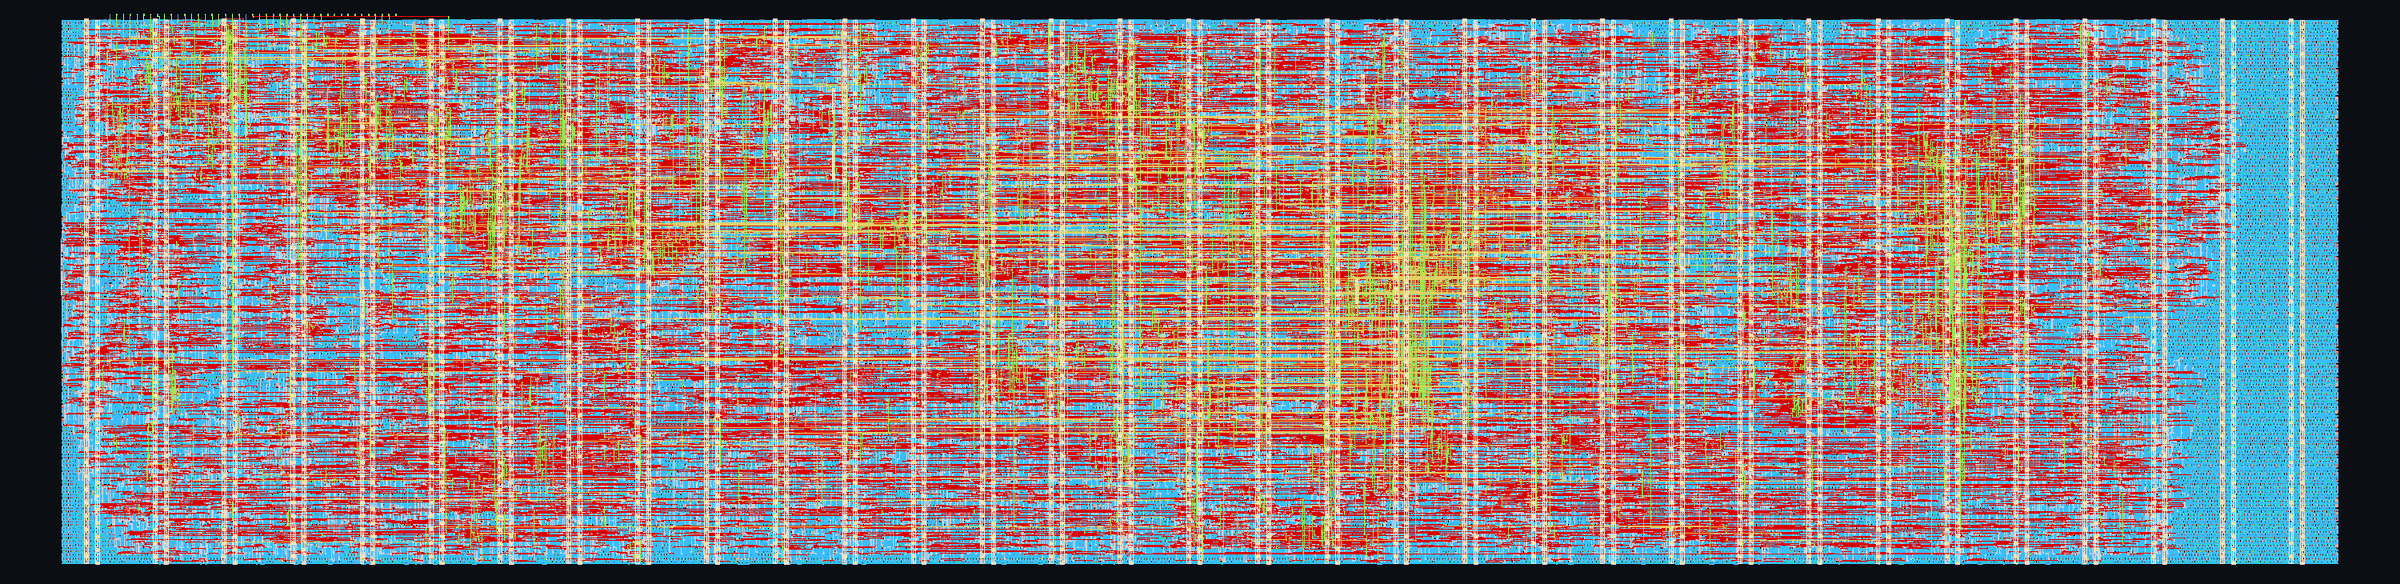
\includegraphics[width=\linewidth]{layout_full.png}\\[2pt]
{\small Routed layout, 6 $\times$ 2 tiles.}
\end{center}

\subsection{Pin map}

\begin{center}
\begin{tabularx}{\linewidth}{@{}llX@{}}
\toprule
Pin & Direction & Use \\
\midrule
\sig{ui[0]} & in & RX: instructions from the host (first byte \sig{0x55}) \\
\sig{uo[0]} & out & TX: data and status to the host \\
\sig{uo[1]} & out & BAUD\_LOCKED \\
\sig{uo[2]}, \sig{uo[3]} & out & ARMED for channels A and B \\
\sig{uo[4]}, \sig{uo[5]} & out & HOST\_FULL for channels A and B \\
\sig{uo[6]}, \sig{uo[7]} & out & SELECT (chip select) for channels A and B \\
\sig{uio[0]}--\sig{uio[2]} & in/out & pins 0--2, driven by channel A: data, pair, clock \\
\sig{uio[3]}--\sig{uio[5]} & in/out & pins 3--5, driven by channel B: data, pair, clock \\
\sig{uio[6]}, \sig{uio[7]} & in & pins 6 and 7 \\
\sig{ui[7:1]} & in & unused \\
\bottomrule
\end{tabularx}
\end{center}

The \sig{PIN} fields count the \sig{uio} pads. Every pad is read back through \sig{pin\_in}, so open-drain I\textsuperscript{2}C and the USB pair work on single pads; a channel drives its pads only when \sig{OUT} enables them.

\section{Limits and future work}

\begin{enumerate}
\item \textbf{Return link bandwidth.} Two bytes per host entry. At 4 clocks per bit the link keeps up with USB low speed and the clocked standards. Full-size 10BASE-T frames (64 bytes and more) arrive faster; they are received but overflow the 16-entry buffer and are reported with the overflow flag.
\item \textbf{Transmit packet size.} The host FIFO holds 8 entries and the instruction link is slow, so a transmitted packet is what the write blocks hold plus 8 \sig{DATA} entries (about 14 bytes).
\item \textbf{Head-of-line blocking.} A host entry waiting for the return link holds up the wire entries behind it. I\textsuperscript{2}C just stretches SCL; a timed transmit would pause.
\item \textbf{Manchester limits.} Receive needs at least 5 clocks per bit (50\,MHz for 10BASE-T); transmit needs an even divider (40 or 60\,MHz).
\item \textbf{Not supported yet.} I\textsuperscript{2}C target mode (needs a branch on the received R/W bit and a START/STOP detector); a read header that captures any value (for the USB PID); CRC generation on chip.
\item \textbf{Reset.} \sig{CLEAR} resets a channel through its asynchronous reset (\sig{rst\_n \&\& !clear}), driven from a control-unit flip-flop.
\end{enumerate}

\section{Files}

\begin{center}
\begin{tabularx}{\linewidth}{@{}l>{\raggedright\arraybackslash}X@{}}
\toprule
Folder or file & Content \\
\midrule
\sig{info.yaml} & Tiny Tapeout project file: title, tile count, source list, pin names \\
\sig{src/top/} & \sig{tt\_um\_vertrex\_star\_proem.sv} (Tiny Tapeout top level and pin map), \sig{protocol\_emulator.sv} (chip core) and \sig{protocol\_emulator\_inst.sv} (instantiation template) \\
\sig{src/core/} & \sig{emulator\_channel}, \sig{control\_unit}, \sig{line\_codec}, \sig{entry\_dispatch}, \sig{return\_path} \\
\sig{src/core/frame\_chain/} & \sig{frame\_chain} and its blocks: \sig{first\_counter}, \sig{header\_counter}, \sig{start\_router}, \sig{main\_counter}, \sig{end\_counter}, \sig{watchdog} \\
\sig{src/primitives/} & Reusable building blocks: \sig{uart\_rx}, \sig{uart\_tx}, \sig{host\_fifo}, \sig{frame\_buffer} \\
\sig{src/files.f} & File list in compile order, used by the scripts \\
\sig{src/config.json} & LibreLane settings for the Tiny Tapeout GDS flow \\
\sig{test/} & cocotb test bench (\sig{tb.v}, \sig{test.py}) for the RTL and the gate-level netlist \\
\sig{sim/} & Test bench \sig{bench.h} and the tests \sig{t\_*.cpp} \\
\sig{scripts/} & \sig{run.sh} (every test, then synthesis), \sig{sta.sh} (timing) \\
\sig{docs/} & This document, the ISA reference, the architecture diagram and its generator \\
\bottomrule
\end{tabularx}
\end{center}

\sig{bash scripts/run.sh} needs Yosys and g++. Setting \sig{LIBERTY} to an IHP liberty file also reports area. Every source file starts with a header giving the file, module, type (top level, core RTL or primitive), place in the hierarchy and submodules. The RTL is SystemVerilog 2008 in the project's coding style, checked with Yosys, Verilator and Icarus Verilog; it has not yet been compiled in Quartus.

\end{document}
